% Abstract for the Spin the Web Book

\chapter*{Abstract}
\addcontentsline{toc}{chapter}{Abstract}

\textbf{Spin the Web} is a framework for building enterprise web portals that serve as "virtualized companies" and addresses the growing challenge of integrating disparate enterprise systems—ERPs, CRMs, BPMSs, and MRPs—into unified, role-based digital channels. This concept addresses a gap in current web technologies.

The framework is built upon three core pillars:

\begin{enumerate}
\item \textbf{The Webbase Description Language (WBDL)}: A declarative language for modeling portal structure, content, and behavior using XML Schema and JSON Schema specifications.

\item \textbf{The Web Spinner}: A server-side engine that interprets webbases (modular portal definitions written in WBDL) to dynamically generate personalized user experiences with real-time content delivery and role-based authorization.

\item \textbf{The Spin the Web Studio}: A webbaselet for editing webbases, enabling direct, in-place modification of portal structures and content. Spin the Web Studio is used as a laboratory for testing the Web Spinner's capabilities.
\end{enumerate}

The project introduces innovative concepts including:
\begin{itemize}
\item \textbf{Webbaselets}: Modular, self-contained WBDL fragments that enable seamless integration of enterprise systems
\item \textbf{Webbase Placeholders Language (WBPL)}: A security-conscious templating engine for dynamic query generation
\item \textbf{Webbase Layout Language (WBLL)}: A component-based rendering system for responsive user interfaces
\item \textbf{Virtualized Company Paradigm}: Portals that provide unified interfaces for diverse stakeholders including customers, employees, suppliers, and partners
\end{itemize}

\begin{figure}[h]
\centering
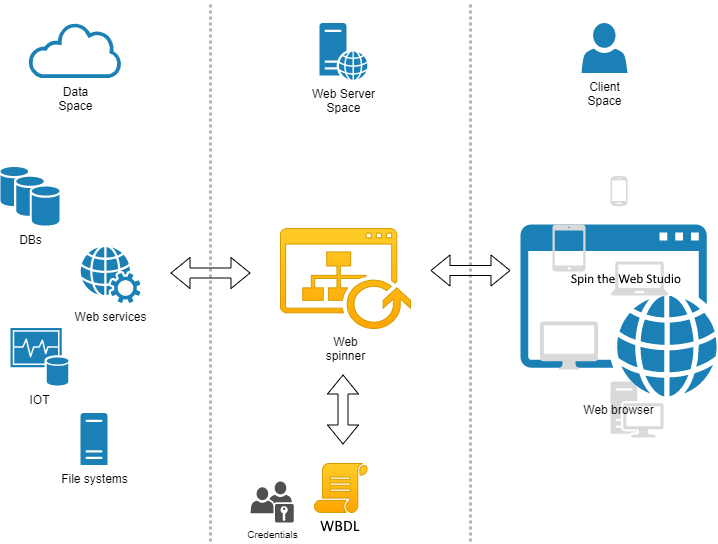
\includegraphics[width=0.7\textwidth]{figures/spin-the-web.png}
\caption{Spin the Web}
\label{fig:spin-the-web}
\end{figure}

This book provides both theoretical foundations and practical implementation guidance, making it suitable for full-stack developers, enterprise architects, and technology leaders responsible for modernizing organizational digital infrastructure. Through detailed examples, best practices, and comprehensive reference materials, readers will gain the knowledge needed to build next-generation web portals that transform how organizations interact with their stakeholders.

The target audience includes professional developers seeking to understand enterprise portal development, system integrators working with complex business requirements, and technology decision-makers evaluating solutions for digital transformation initiatives.

Project repository: \url{https://github.com/keyvisions/spintheweb}.

\clearpage
